\chapter{Motivation}\label{motivation}
Der stetig steigende Fachkräftemangel trifft auch das Baugwerbe. 
Laut einer Umfrage des Hauptverbandes der Deutschen Bauindustrie e.V. stufen über 75 Prozent aller befragten Unternehmen sowohl den vorherrschenden Fachkräftemangel, als auch die steigenden Energie- und Rohstoffpreise als Risiko für das eigene wirtschaftliche Wachstum ein \cite{Bauindustrie:online}.
Abbildung \ref{fig:Fachkräftemangel} illustriert die Entwicklung dieser Sorge über einen Zeitraum von etwas mehr als zwanzig Jahren.
Damit ist es wenig überraschend, dass eine Bewegung weg von menschlichen Arbeitskräften hin zur Automatisierung existiert.
Neben dem Fachkräftemangel stellt aber auch die geringe Effizienz von Bauvorhaben ein Problem dar, welche sich über den gesamten Planungs- und Bauprozess erstreckt. 
Diese Ineffizienz entsteht aufgrund der Vielzahl der an Bauprojekten beteiligten Experten und Unternehmen und ist, als \textit{Fragmentierungsproblem der Bauindustrie} bezeichnet, ein bekanntes Problem  \cite{ConstructionFragmentation}.
\begin{figure}[h]
    \centering
    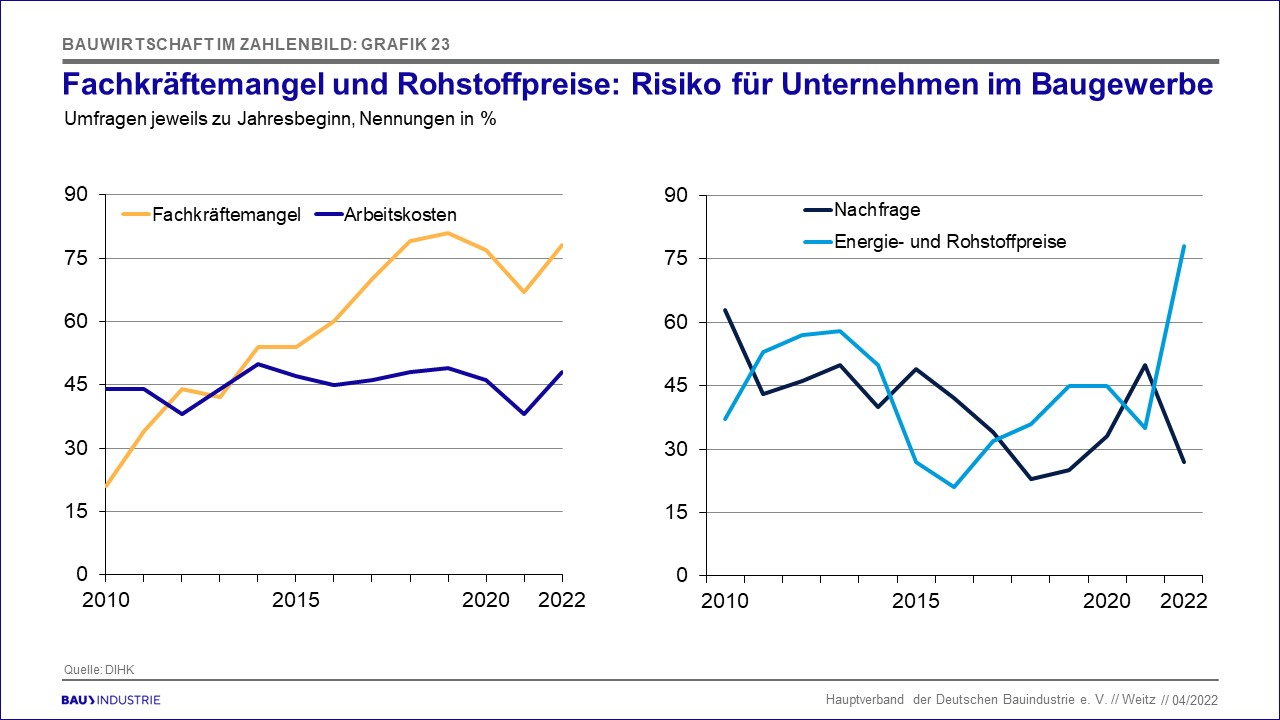
\includegraphics[width=0.7\columnwidth]{fig/Grafik_23.jpg}
    \caption{Während wirtschaftliches Risiko durch eine potentiell sinkende Nachfrage nach Bauafträgen und eventuell steigender Arbeitskosten unverändert blieben oder sogar als weniger relevant bewertet wurden, ist ein deutlicher Anstieg aufgrund des vorherrschenden Fachkräftemangels und der Energie- und Rohstoffpreise zu erkennen.}
    \label{fig:Fachkräftemangel}
\end{figure}
Deshalb etablieren sich derzeit Standards, um Bauprojekte digital zu begleiten.
Mit diesen soll gleichzeitig die Effizienz gesteigert, die Kommunikation zwischen den einzelnen Expertenteams vereinfacht, der Arbeitsplatz "Baustelle" sicherer gestaltet und ein resourcensparender Bau ermöglicht werden \cite{BIMforHe12:online} \cite{Top10Ben31:online}.
Gleichzeitig steigen mit der Zunahme an digitalen Informationen zu Bauprojekten, auch die Möglichkeiten diese besser zu analysieren, zu optimieren und an neue Technologien zu knüpfen.
Erst dadurch wurde das seit einigen Jahren erforschte Gebiet der Additiven Fertigung von Gebäuden, etwa mit Beton druckenden Roboterarmen oder mobilen Robotern, realisierbar \cite{AdditiveManufacturingUsingMobileRobots}. [TODO nochmal reinschauen ob das einigermaßen als Quelle passt]. 
Obwohl es mittlerweile viele Projekte zur Additiven Fertigung von Gebäuden gibt, haben diese oft den Nachteil der Nicht-Parallelisierbarkeit der druckenden Roboter, die durch die Höhe der temporären Stützstrukturen (wie Kräne, Gerüste, Aufhängungen) eingeschränkte Bauhöhe und die vergleichsweise lange Bauzeit [TODO Quelle oder lange bauzeit weg].
[Frage wegen Kommentar: Star Wars roboterschwarm/Marsbesiedelung; soll ich hier sagen dass ein derzeit in der SciFi Szene aufgekommener Trend von organisierten Roboterschwärmen, die was bauen gar nicht so blöd ist und wir das ähnlich angehen?]
Diesen Einschränkungen soll nun mithilfe eines Schwarmes bodengebundener automoner Roboter, welche gleichzeitig an dem Bauprojekt arbeiten, entgegengewirkt werden.
Dabei sollen sich die Roboter auf den Mauern des Gebäudes selbst bewegen können, während sie dieses errichten.
In dieser Arbeit liegt der Schwerpunkt allerdings nicht auf dem Entwicklen der Roboter selbst, sondern das Erstellen eines Bauplans für den genannten Roboterschwarm basierend auf einem 3D Modells des Gebäudes.
Das Erstellen des Modells innerhalb eines nutzerfreundlichen 3D Editors stellt nicht nur die geometrischen und physikalischen Eigenschaften des Gebäudes digital bereit, sondern verschlankt auch die Kommunikation zwischen Endnutzer und Architekt oder ersetzt letzteren komplett.
Gleichzeitig bildet diese Arbeit damit  auch den Trend hin zur sogennanten Massenpersonalisierung ab, welcher als Nachfolgetrend zur Massenproduktion und als "heilger Gral" der Fertigung angesehen wird
%[TODO https://link.springer.com/chapter/10.1007/978-3-642-56192-4_4]
.
Dieser Trend ist auch für die Bauindustrie interessant, denn auch hier schafft die Möglichkeit sämtliche 
%[ugs https://link.springer.com/chapter/10.1007/978-3-319-77556-2_34] 
Kundenwünsche an ein Produkt (oder Gebäude) umzusetzen, ohne dafür spezielles Werkzeug herstellen zu müssen, neue Gewinnmöglichkeiten.
Mit der Option der Modellierung des Gebäudes durch den Kunden selbst, ist die Kommunikation mit den Architekten über dessen Wünsche effizienter, da beide Parteien zusammen an dem Modell arbeiten können.
Im Anschluss an den Designprozess des 3D Models des Gebäudes, soll dieses in einen Bauplan übersetzt werden, welcher alle notwendigen Informationen für den oben genannten Roboterschwarm enthält, sodass dieser das Gebäude selbstständig errichten kann [TODO ugs].
Dieses Konzept wird anhand nachfolgender Fallstudie(n) getestet.



